\subsubsection{How are data sources connected?}
\label{subsec:data-source-connections}
The diagrams describe the analytical relationships used throughout this report,
including the executive summary's underlying tables and figures. They do not
assert database-enforced foreign keys or upstream replication lineage. All
physical sources resolve in \texttt{EDLDB}; \texttt{HCDM} abbreviates
\texttt{BT\_HCA\_HCDM}. Blue solid boxes are physical tables or views; amber
dashed boxes are derived datasets. Arrows carry source evidence into a result;
edge labels state join fields and direction, rather than implying cardinality.
The two upload sources are compared independently, without a record-to-record
join between them. The notification source is used in verification, while
the later study figures use HCDM uploads.

\paragraph{How do the report’s source tables and analyses connect?}
Report-wide source connections; details and matching rules follow.

\begin{center}
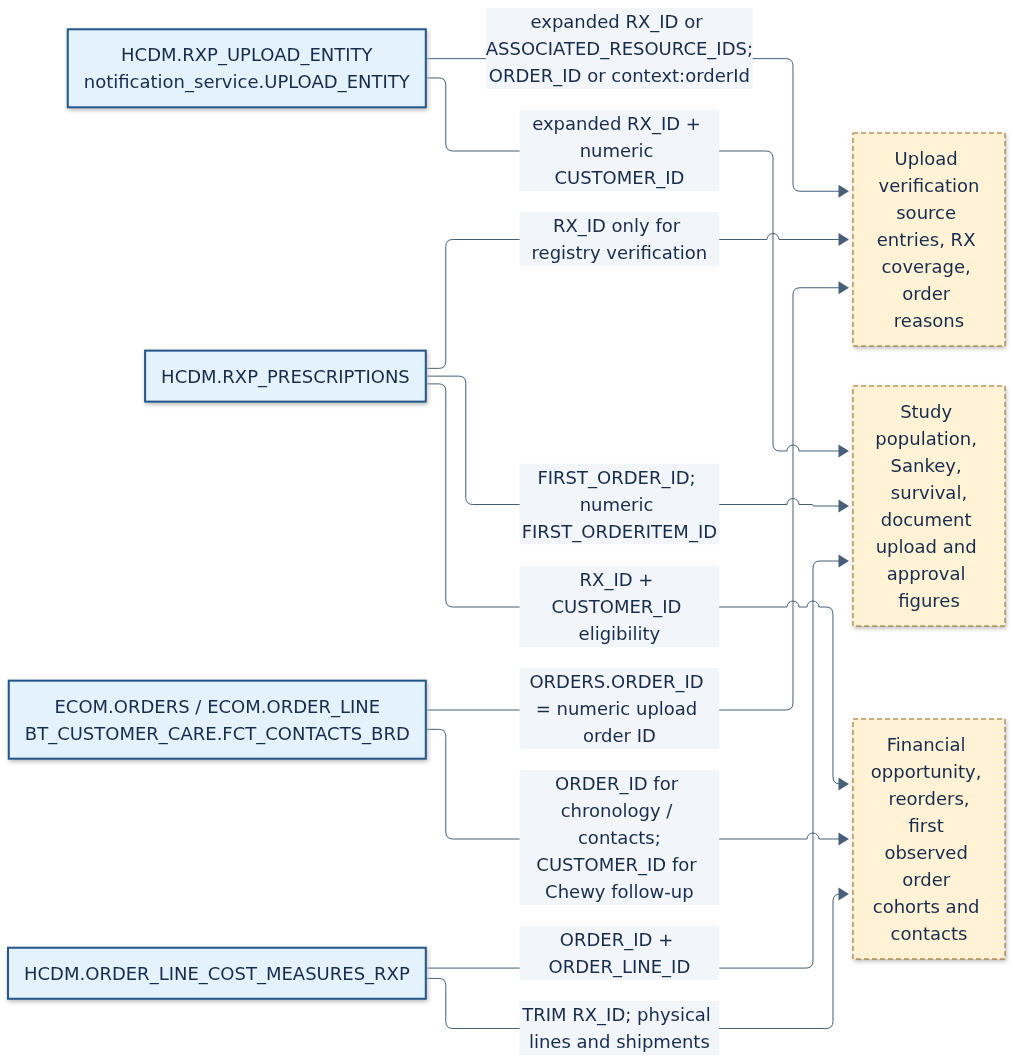
\includegraphics[width=\linewidth,height=0.75\textheight,keepaspectratio]{targets/report-source-overview/outputs/diagrams/visual.png}
\captionof{figure}{Report-wide source connections; details and matching rules follow.}
\label{fig:data-source-overview}
\end{center}




\clearpage
\noindent\textbf{Source grains and counting units.}
\paragraph{What is the grain and counting unit of each source?}
The table below records the source grains and counting units used throughout the analysis.

\begin{longtable}{@{}>{\raggedright\arraybackslash}p{0.36\linewidth}>{\raggedright\arraybackslash}p{0.59\linewidth}@{}}
\toprule
Source (within \texttt{EDLDB}) & Grain used by this report \\
\midrule
\endhead

\texttt{HCDM.RXP\_UPLOAD\_ENTITY} & Physical upload row; entity analyses validate \texttt{UPLOAD\_ID} and count it once, despite multiple expanded prescription IDs. \\

\texttt{RXP\_NOTIFICATION\_SERVICE.}\allowbreak\texttt{UPLOAD\_ENTITY} & Physical upload row; prescription IDs may be a list. Context order and item IDs are separate fields. \\

\texttt{HCDM.RXP\_PRESCRIPTIONS} & Prescription \texttt{RX\_ID}; analyses check uniqueness or consistency of repeated registry values. \\

\texttt{HCDM.ORDER\_LINE\_COST\_}\allowbreak\texttt{MEASURES\_RXP} & Shipment $\times$ physical line: \texttt{ORDER\_ID}, \texttt{ORDER\_LINE\_ID}, \texttt{SHIPMENT\_KEY}. A line can have multiple shipments. \\

\texttt{ECOM.ORDERS} & Order header \texttt{ORDER\_ID}; linked-order verification checks uniqueness, chronology analyses check consistent repeated values. \\

\texttt{ECOM.ORDER\_LINE} & Physical line \texttt{ORDER\_ID}, \texttt{ORDER\_LINE\_ID}; \texttt{NET\_SALES} is already the full line amount. \\

\texttt{BT\_CUSTOMER\_CARE.}\allowbreak\texttt{FCT\_CONTACTS\_BRD} & Contact leg/session evidence, identified by order, \texttt{SESSION\_ID} and \texttt{LEG\_ID} for conflict checks; published counts use distinct customers, orders or relative days. \\
\bottomrule
\end{longtable}



\noindent\textbf{Duplicates and aggregation.}
Source-entry counts and timestamp extrema use all physical upload rows without
deduplication. Prescription verification expands IDs and reduces them to distinct
source/prescription sets, preventing upload multiplicity from multiplying registry
counts. Coverage preserves eligible prescriptions with left joins; the channel
distribution excludes unmatched and non-vet-diet IDs from its denominator.
Order-reason comparisons count each normalized order once per source, retaining
unmatched IDs separately from matched orders whose reason is SQL NULL.
\texttt{context:orderItemId} is audited for presence in the NULL-resource analysis;
it is not a join key for those order-level results.

For first-order figures, shipment rows collapse to one
\texttt{(ORDER\_ID, ORDER\_LINE\_ID)} before prescription association.
Attribute-variant checks prevent conflicting shipment evidence from being silently
resolved by SQL \texttt{MIN}/\texttt{MAX}. Multiple prescription associations
are retained for audit, then distinct prescriptions, orders or lines are counted
according to each output's grain. Missing or invalid first-order keys are audited
outside the matched-line denominator. The decision extract uses an inner join
because it describes matched first-order populations only.

Financial calculations instead retain one amount per distinct
\texttt{(ORDER\_ID, ORDER\_LINE\_ID, SHIPMENT\_KEY)} and sum shipments to lines;
identical amounts on different shipments remain separate contributions.
Repeated associations cannot multiply sales. The baseline includes only shipment
or cancellation records in its reporting window. Chewy-wide follow-up uses
\texttt{ECOM.ORDER\_LINE.NET\_SALES} once per line, without summing it as
shipment data. Consistent duplicates may collapse; conflicting key values fail
the relevant generator's validation. Totals count distinct customers and orders
again, rather than adding overlapping category counts.

\clearpage
\noindent\textbf{Upload verification joins.}
The channel and coverage tables match normalized prescription ID only, with no
customer, upload-date or order restriction. The coverage cohort applies its
registry creation cutoff and vet-diet/customer-upload filters; the channel
comparison covers all uploaded vet-diet prescriptions. Numeric order IDs require
trimmed digits before conversion. Source-order extracts are merged in Python
with validated ECOM order headers using a left join.
\paragraph{How are upload IDs expanded and matched to prescriptions and orders?}
Upload-source prescription expansion, registry matching and context-order matching.

\begin{center}
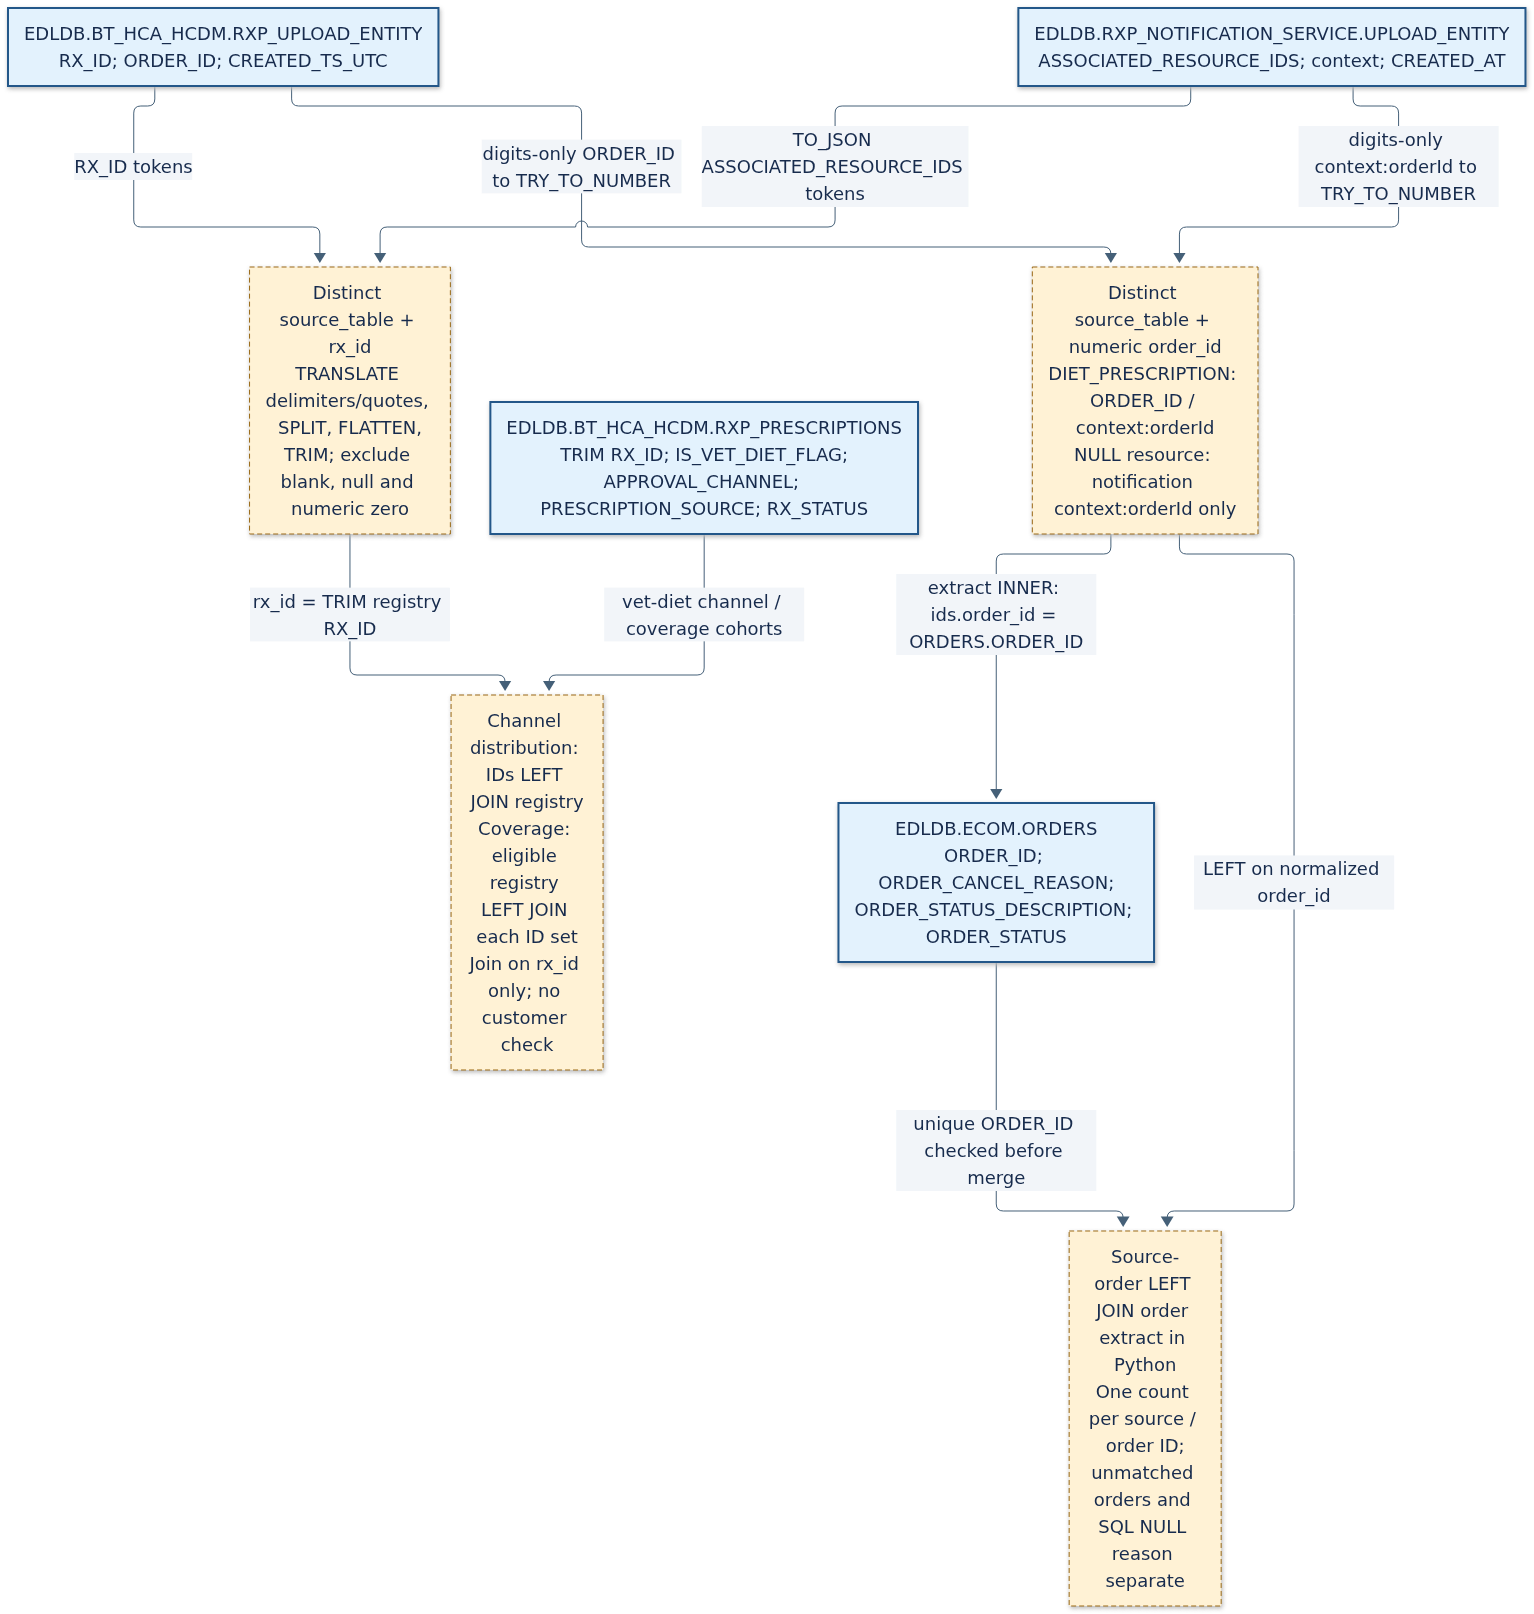
\includegraphics[width=\linewidth,height=0.76\textheight,keepaspectratio]{targets/upload-verification-joins/outputs/diagrams/visual.png}
\captionof{figure}{Upload-source prescription expansion, registry matching and context-order matching.}
\label{fig:data-source-upload-verification}
\end{center}




\clearpage
\noindent\textbf{Prescription, first-order and upload evidence.}
The study population uses CMPU vet-diet prescriptions created August 15 through
October 14, 2026, UTC; focused figures also require
\texttt{APPROVAL\_CHANNEL = CUSTOMER\_UPLOAD}. Both first-order keys are required:
\texttt{FIRST\_ORDER\_ID = ORDER\_ID} and the digits-only numeric conversion of
\texttt{FIRST\_ORDERITEM\_ID = ORDER\_LINE\_ID}. Upload matching additionally
requires registry \texttt{CUSTOMER\_ID} to equal the numeric upload customer ID.
\paragraph{How are prescriptions matched to first-order lines and upload evidence?}
First-order line matching and two distinct ways of selecting upload evidence.

\begin{center}
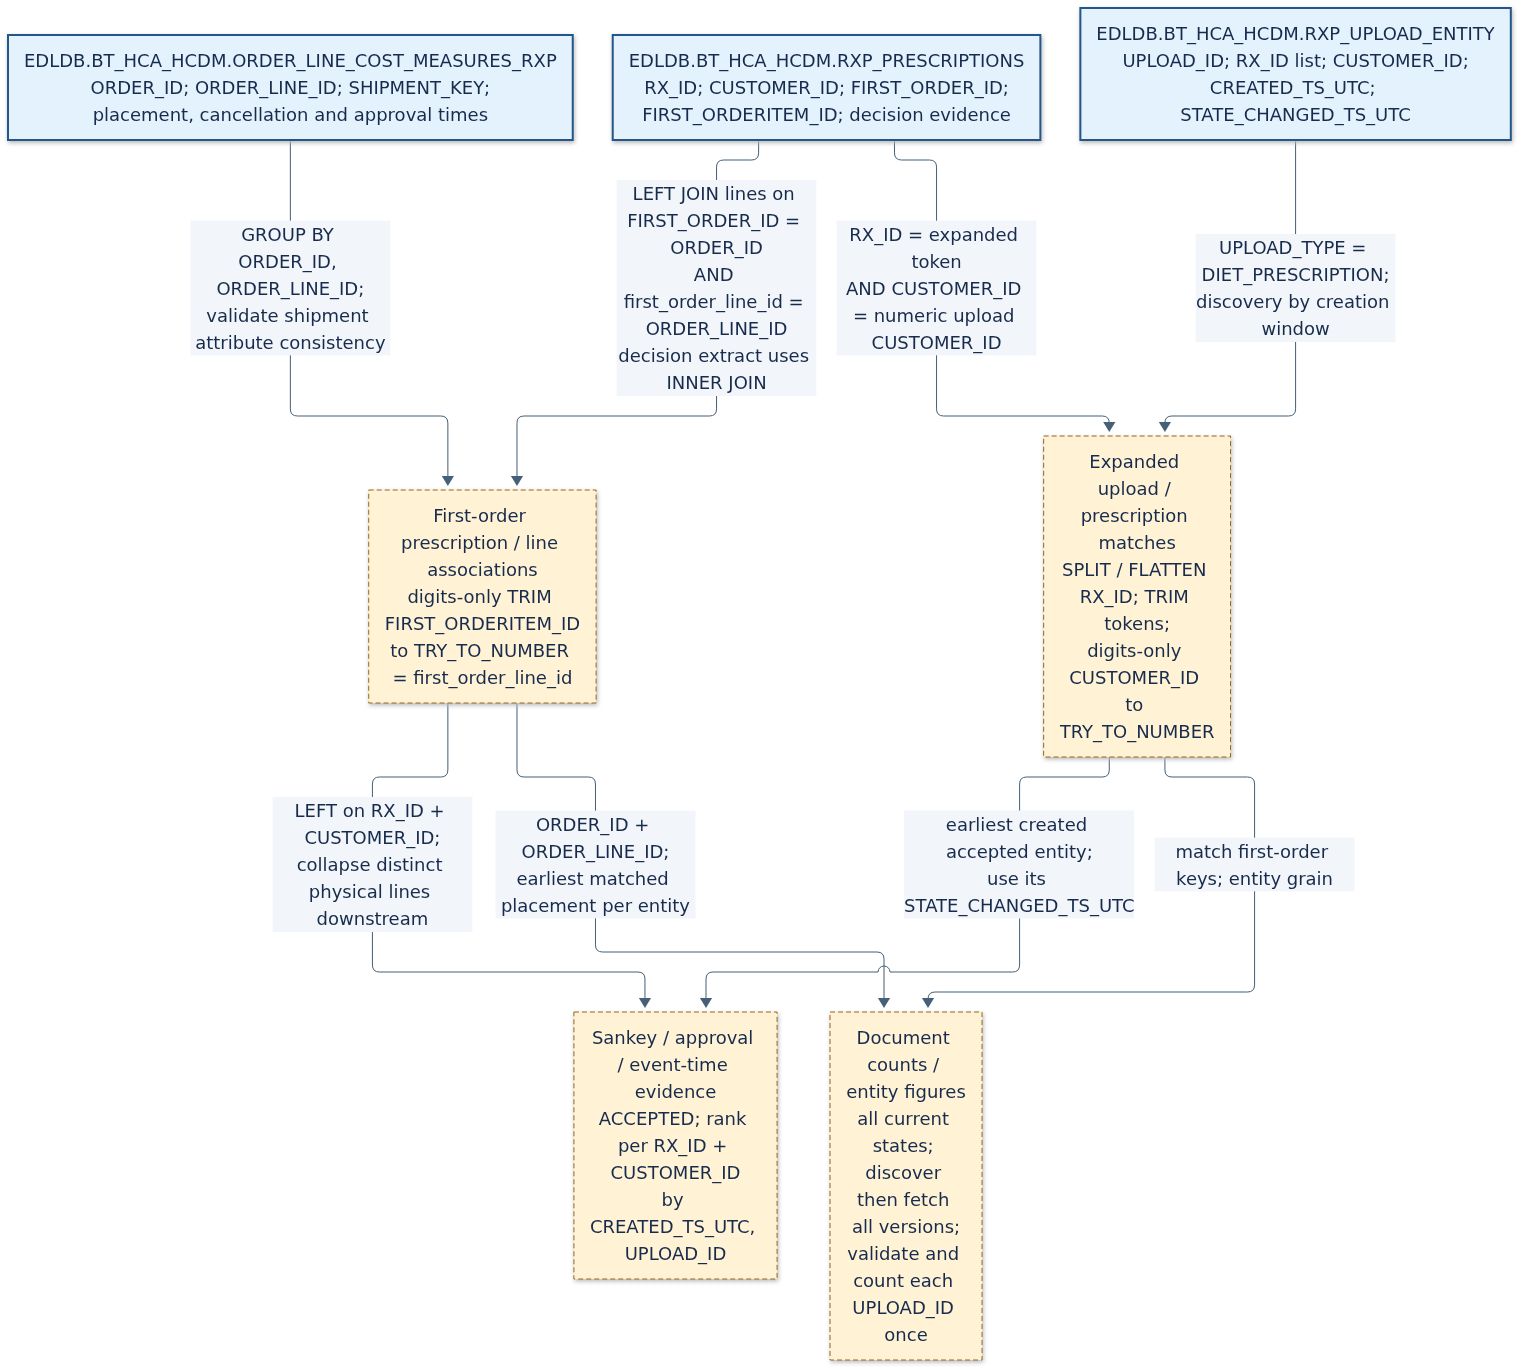
\includegraphics[width=\linewidth,height=0.69\textheight,keepaspectratio]{targets/prescription-first-order-joins/outputs/diagrams/visual.png}
\captionof{figure}{First-order line matching and two distinct ways of selecting upload evidence.}
\label{fig:data-source-first-order}
\end{center}




\clearpage
\noindent\textbf{Selection and observation windows.}
The Sankey, approval and survival pipelines select the earliest-created currently
\texttt{ACCEPTED} upload per prescription/customer, breaking ties by
\texttt{UPLOAD\_ID}; the measured upload time is that entity's
\texttt{STATE\_CHANGED\_TS\_UTC}, not its creation time. Survival selects the
earliest-created associated entity again at line grain. Approval comparisons use
the line's \texttt{MAX\_APPROVED\_DATETIME}; survival uses
\texttt{MIN\_APPROVED\_DENIED\_DATETIME} for its 96\% interval estimate when actual
upload time is unavailable, then compares the candidate with cancellation.
These estimates are derived events, not extra source tables.

Entity-state figures and document counts retain all current states, discover
entities by creation time, fetch all versions of discovered IDs to expose
conflicts, and count each entity once. The order-relative entity figure uses
its earliest populated matched first-order placement. Upload discovery starts
August 1; the Sankey/approval/entity figures use an exclusive October 26 bound,
while survival uses an exclusive October 27 bound. Unknown creation times are
retained for entity auditing. Current state changes and prescription decisions
can occur after the discovery or aged-cancellation cutoff; these are snapshots,
not historical event streams.

The study's first-versus-all-order comparison additionally matches
\texttt{TRIM(line.RX\_ID) = prescription.RX\_ID} and customer ID for all linked
orders, without an order-placement window. Its frozen physical keys are passed
to \texttt{prescription\_cohort\_order\_sales.sql} for shipment financial enrichment
on both order and line ID. This differs from joining only
\texttt{FIRST\_ORDER\_ID}. Decision evidence comes from the registry plus the
matched line's approval/denial fields; no separate decision table is joined.

\noindent\textbf{Financial, reorder and contact rules.}
The financial baseline's SQL left-joins the registry on trimmed line
\texttt{RX\_ID}; Python then requires nonmissing, equal numeric customer IDs and
the CMPU/vet-diet/customer-upload flags. Aged-anchor queries apply these same
customer and prescription checks directly in SQL. The baseline's shipped-or-cancelled
window and the anchors' cancellation window are May 1 inclusive to August 1
exclusive, 2026; they do not impose the study's prescription-creation window.

First observed vet-diet and first customer-upload vet-diet cohorts use RxP line
history, then ECOM order headers by order and customer ID. Chronology ranks by
placement then order ID; earliest-time ties, missing placements and missing
headers are audited and excluded from unambiguous first-order cohorts. Vet-diet
history uses line vet-diet flags without requiring a registry match;
customer-upload history also matches registry prescription/customer IDs and
restricts that channel. Both histories span all prescription sources and dates. This is observed
history, not a claim of complete lifetime coverage.


\paragraph{How are financial lines, later orders, and customer contacts connected?}
Financial eligibility, order chronology, reorder matching and contact matching.

\begin{center}
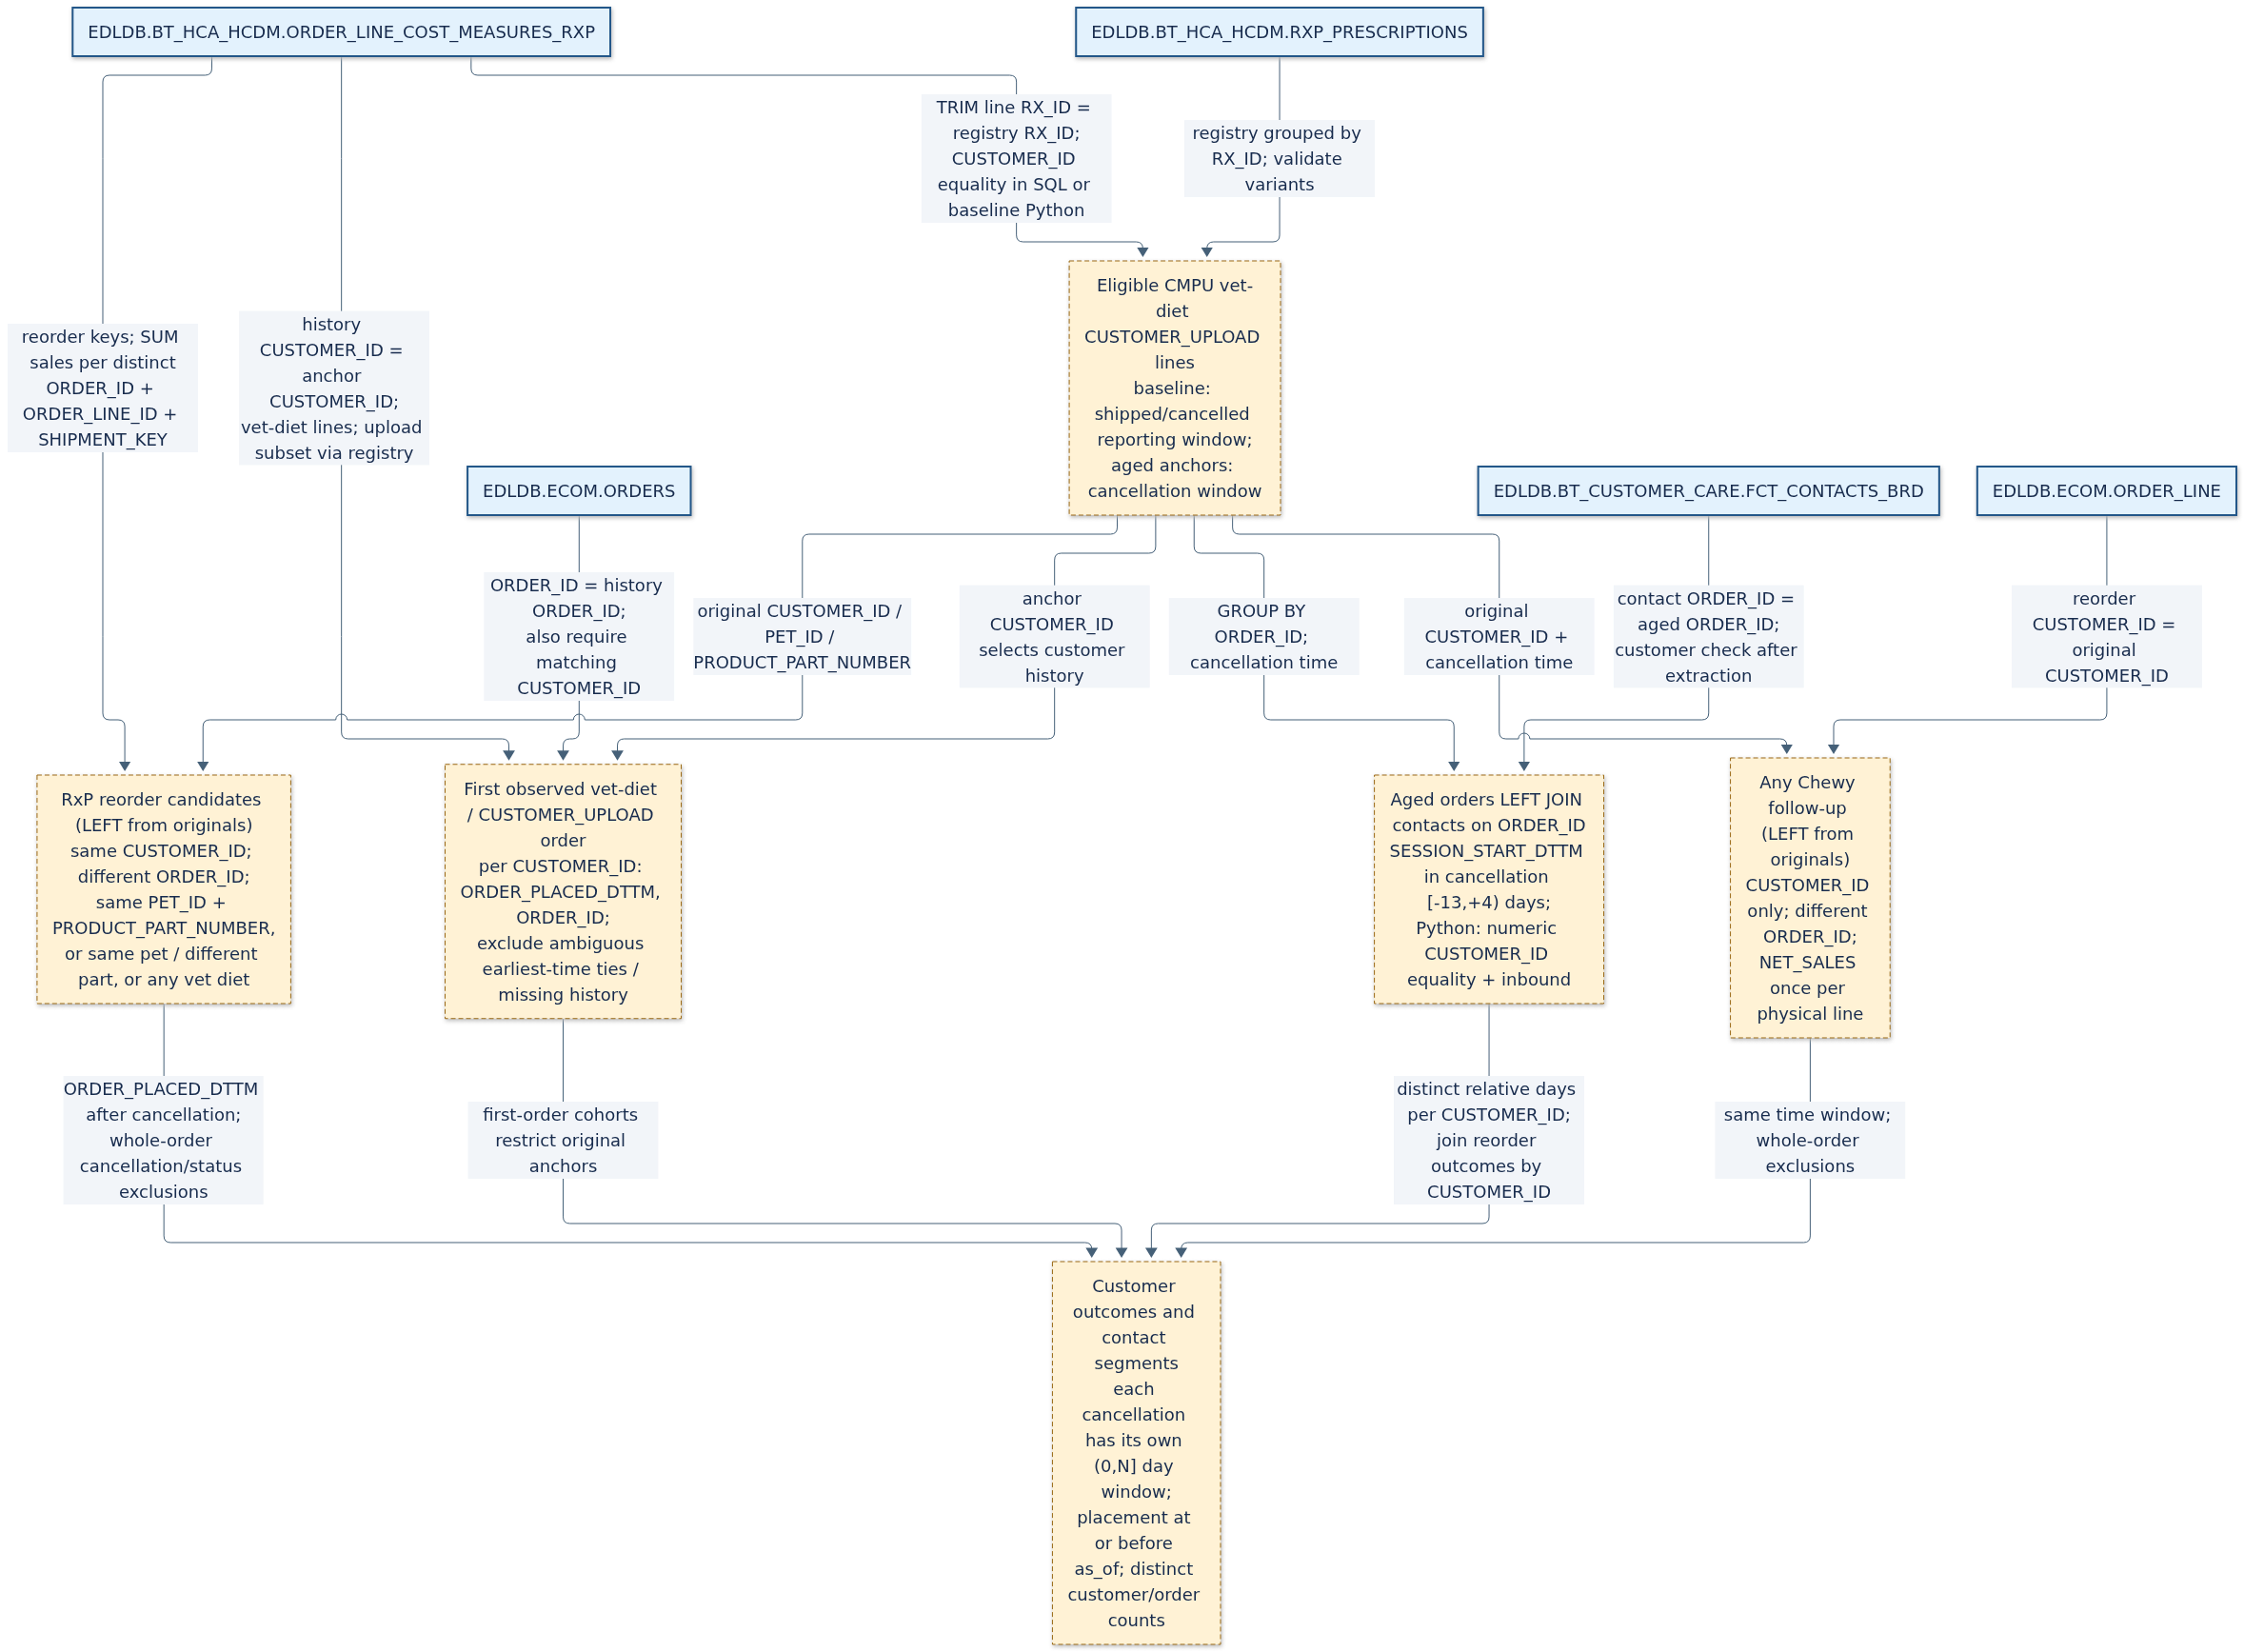
\includegraphics[width=\linewidth,height=0.88\textheight,keepaspectratio]{targets/financial-reorder-contact-joins/outputs/diagrams/visual.png}
\captionof{figure}{Financial eligibility, order chronology, reorder matching and contact matching.}
\label{fig:data-source-financial}
\end{center}





RxP follow-up matches exact customer, non-null pet and nonblank product part
number for the same-product endpoint. Its other endpoints use the same pet with
a different part, or any vet-diet line for that customer. Chewy-wide follow-up
matches customer only in \texttt{ECOM.ORDER\_LINE}. All endpoints require a
different order placed strictly after its matched cancellation and through
the specified follow-up day inclusive, bounded by the October 28, 2026,
00:00 UTC observation cutoff. Windows of 7--70 days overlap; each cancellation
is its own anchor. Whole candidate orders with cancellation evidence or unknown
line status are excluded. Orders and sales are deduplicated across repeated
anchor matches; a reordering customer counts once within each endpoint/window.

Contacts join the original aged order on \texttt{ORDER\_ID} in SQL; Python
normalizes identifiers and additionally requires equal nonmissing customer IDs,
inbound direction and a populated timestamp. Contact legs are checked for
conflicts and exact duplicate rows collapse. Relative days are elapsed UTC
24-hour bins, from $[-13,+4)$ days around cancellation, rather than calendar
dates. The report includes handled, unhandled and unknown-handled inbound
attempts. Frequency counts distinct relative days across a customer's aged
orders. The contact-frequency and $-7$ through $+3$ contact-window comparisons
join customer-level segments to verified 14-day same-pet/part outcomes by
\texttt{CUSTOMER\_ID}, retaining customers without a reorder in the denominator.

Table~\ref{tab:customer-contacts-by-cancellation-reason} uses the broader financial
shipment/cancellation cohort and the same contact order/customer joins, grouping
distinct contacting customers by current reason. No creation-relative day bounds
apply; contacts are capped at the latest observed shipment/cancellation
event per order and reason. Its SQL and generator are
\path{src/sql/opportunity_customer_contacts_by_cancel_reason.sql} and
\path{src/python/create_opportunity_contacts_by_cancel_reason.py}.

Figure~\ref{fig:data-source-contact-matching} isolates the contact-matching
pipeline, including the customer checks applied after the SQL extraction.

\paragraph{How are customer contacts matched to aged orders and observation windows?}
Contact matching: aged-order eligibility, SQL order/time join, Python customer checks and distinct counting.

\begin{center}
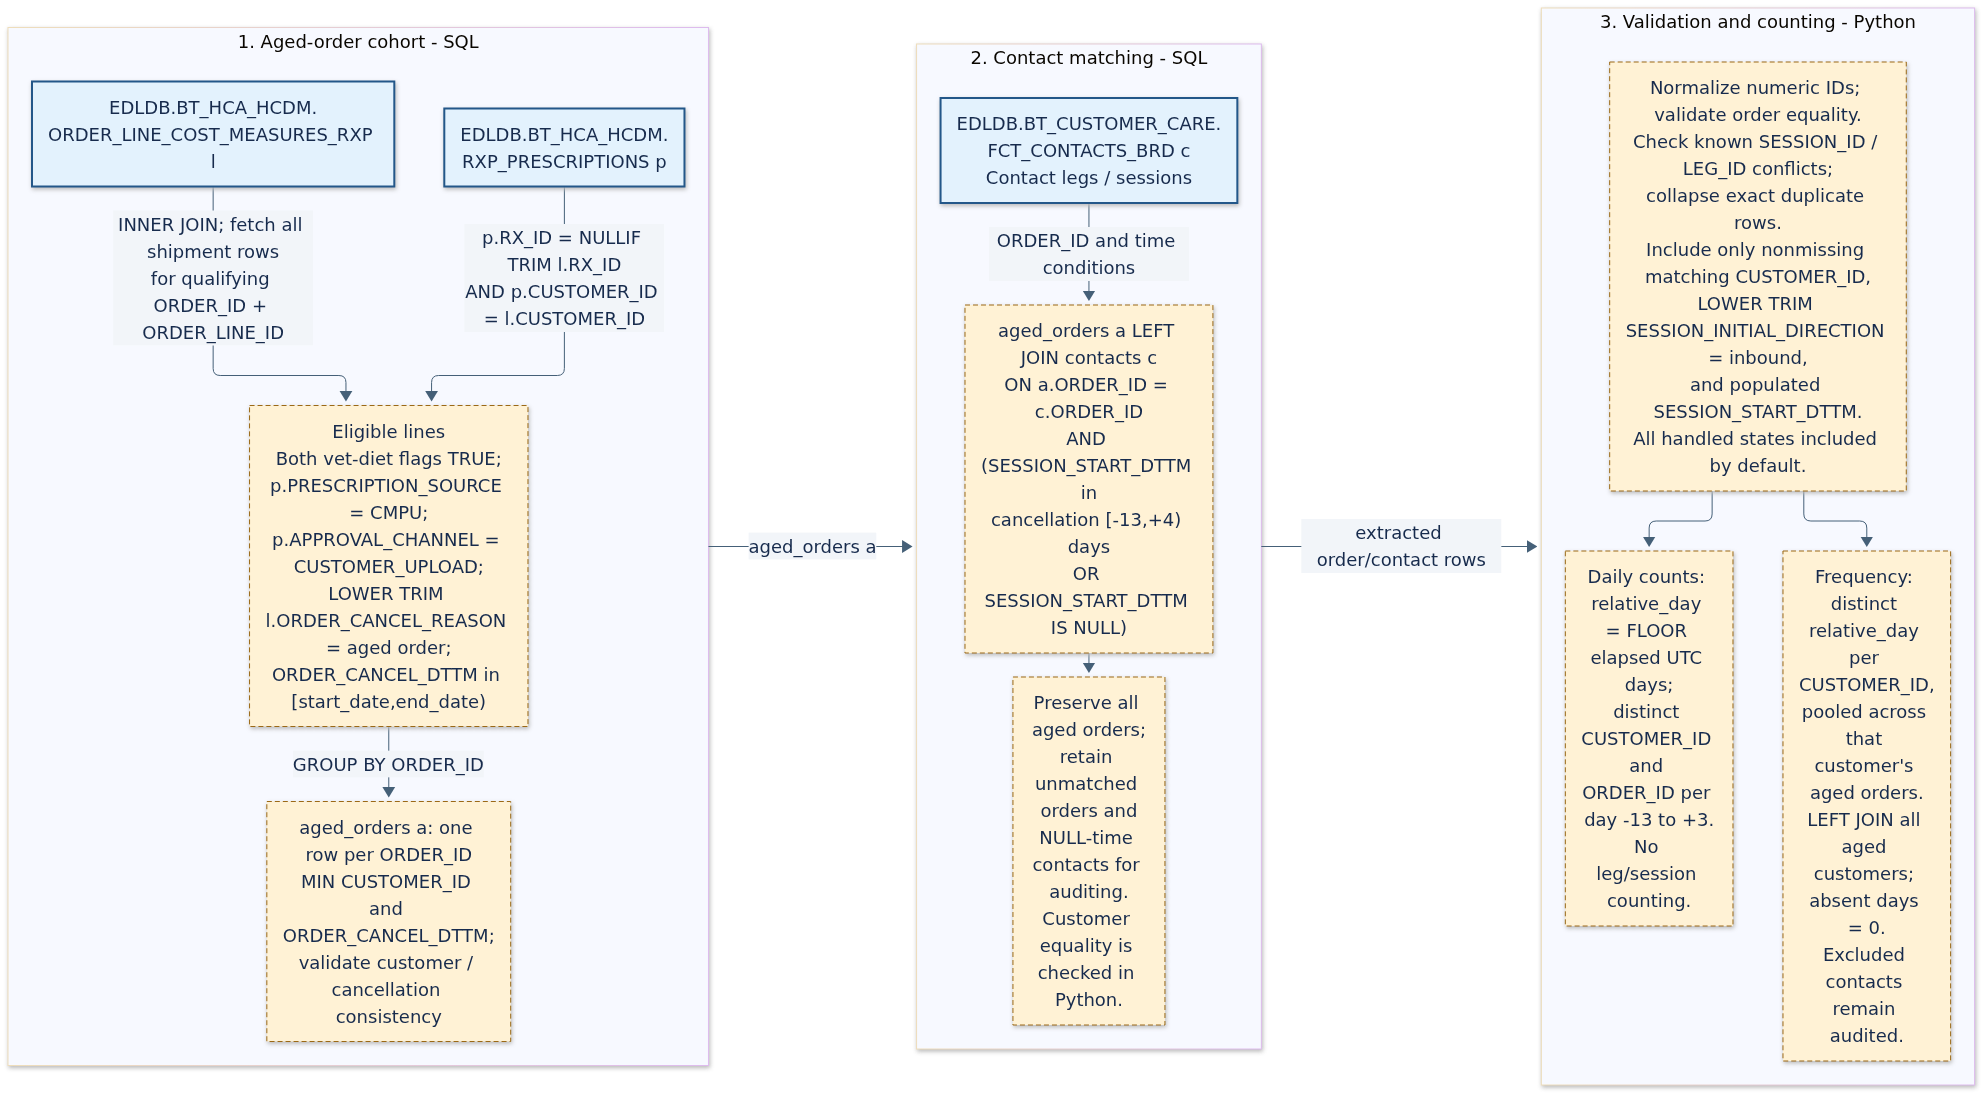
\includegraphics[width=\linewidth,height=0.88\textheight,keepaspectratio]{targets/contact-matching-rules/outputs/diagrams/visual.png}
\captionof{figure}{Contact matching: aged-order eligibility, SQL order/time join, Python customer checks and distinct counting.}
\label{fig:data-source-contact-matching}
\end{center}





\noindent\textbf{Reproduction and source trace.}
Run \texttt{make data-source-diagrams} to generate the editable Mermaid sources
and transparent PNGs; \texttt{make report} also rebuilds missing or outdated
diagrams. The tracked definitions are in
\path{src/python/create_data_source_diagrams.py}; the Markdown grain table is
\path{outputs/tables/data-source-connections/source-grains.md}.
The following implementation files define the relationships above; independently
aggregated verification SQL checks the same populations without adding sources.
Unused exploratory queries are excluded from this map.
\begin{itemize}
\item Verification: \path{src/sql/upload_data_verification.sql},
\path{upload_source_time_coverage.sql},
\path{upload_vet_diet_approval_channels.sql},
\path{cmpu_approved_prescription_upload_coverage.sql},
\path{diet_upload_source_orders.sql}, \path{diet_upload_linked_orders.sql},
\path{null_resource_upload_context.sql} and \path{null_resource_upload_orders.sql}
(all under \path{src/sql/}); their corresponding \path{src/python/analyze_*.py}
modules validate and merge the retained extracts.
\item Study figures: \path{src/sql/cmpu_first_order_line_status.sql},
\path{cmpu_first_order_line_event_times.sql},
\path{cmpu_first_order_line_approval_distribution.sql},
\path{cmpu_upload_to_max_approval_extract.sql},
\path{cmpu_upload_entity_state_change_distributions.sql},
\path{cmpu_upload_entity_order_creation_distributions.sql},
\path{cmpu_study_population_uploaded_documents.sql} and
\path{cmpu_study_population_prescription_decisions.sql}; the corresponding
\path{src/python/create_cmpu_*.py} modules enforce line/entity grains.
The frozen all-order membership query is retained under
\path{data/opportunity/prescription-cohort-orders/}; financial enrichment uses
\path{src/sql/prescription_cohort_order_sales.sql}.
\item Financial and contacts: \path{src/sql/opportunity_order_cancellation_summary.sql},
\path{opportunity_aged_reorders.sql},
\path{opportunity_new_upload_customer_follow_up.sql},
\path{opportunity_new_vet_diet_customer_follow_up.sql}, and the three
\path{opportunity_*chewy_follow_up.sql} templates;
\path{opportunity_aged_first_vet_diet_order_customers.sql},
\path{opportunity_aged_first_customer_upload_vet_diet_order_customers.sql} and
\path{opportunity_aged_customer_contacts.sql} define history and contact extracts.
The corresponding opportunity Python generators aggregate outcomes;
\path{src/python/create_opportunity_contact_frequency_reorders.py} combines
contact segments and reorder outcomes. Retained rendered queries, source
fingerprints and local verification SQL are under \path{data/opportunity/}.
\end{itemize}
\clearpage

